\documentclass[conference]{IEEEtran}
\IEEEoverridecommandlockouts
% The preceding line is only needed to identify funding in the first footnote. If that is unneeded, please comment it out.
\usepackage{cite}
\usepackage{amsmath,amssymb,amsfonts}
\usepackage{algorithmic}
\usepackage{graphicx}
\usepackage{textcomp}
\usepackage{xcolor}
\def\BibTeX{{\rm B\kern-.05em{\sc i\kern-.025em b}\kern-.08em
    T\kern-.1667em\lower.7ex\hbox{E}\kern-.125emX}}

% \documentclass{article}

\usepackage{hyperref} %BUG if put after
\usepackage{tikz}
\usetikzlibrary{calc,shapes,positioning}
\usetikzlibrary{arrows}
\newcommand{\midarrow}{\tikz \draw[-triangle 90] (0,0) -- +(.1,0);}
% Be sure to use PDxF Latex
\pdfoutput=1

% \usepackage[latin1]{inputenc}

\usepackage{url}
% \usepackage{fullpage}
\usepackage{cite}
\usepackage{caption}
\usepackage{bm}
\newcommand{\ubar}[1]{\mkern2mu\underline{\mkern-2mu #1\mkern-2mu}\mkern2mu}
% \allowdisplaybreaks
\usepackage{mystyle}


\usepackage{amsmath,graphicx}
% format A4
% \usepackage{vmargin}
% \setpapersize{A4} 

\RequirePackage{algorithm}
\RequirePackage{algorithmic}

% Attempt to make hyperref and algorithmic work together better:
% \newcommand{\theHalgorithm}{\arabic{algorithm}}

\hypersetup{  
  bookmarks=true,
  backref=true,
  pagebackref=false,
  colorlinks=true,
  linkcolor=blue,
  citecolor=red,
  urlcolor=blue,
  pdftitle={alphaBP},
  pdfauthor={Dong Liu},
  pdfsubject={}
}


\begin{document}
\title{$\alpha$ Belief Propagation as Fully Factorized Approximation}
\author{
  \IEEEauthorblockN{
  Dong Liu, Nima N. Moghadam, Lars~K. Rasmussen, Jinliang Huang, Saikat Chatterjee}

% \IEEEauthorblockA {$^{1}$ KTH Royal Institute of   Technology, Stockholm, SE-100~44, Sweden.\\
%   (e-mail: \{doli, lkra, sach\}@kth.se)} \\
% \IEEEauthorblockA {$^{2}$ Huawei Technologies Sweden AB\\
%   Stockholm, Sweden.\\
%   (e-mail: \{jinliang.huang, nima.najari.moghadam1\}@huawei.com)}

}
% \address[2]{Huawei}
% \name{
% Dong Liu,
% Minh Th�nh Vu,
% Saikat Chatterjee,
% and Lars~K. Rasmussen
% }

%   \address{
%   KTH Royal Institute of Technology, Stockholm, Sweden 
%   E-mail: \{doli\}@kth.se}



\maketitle
\begin{abstract}
This work follows Minka's work \cite{divergence-measures-and-message-passing} and obtains $\alpha$ Belief Propagation ($\alpha$-BP), which generalizes standard BP. $\alpha$-BP can be interpreted as approximating a distribution $p$ by a fully factorized distribution $q$. Then the Bayesian inference problems on $p$ (usually computational expensive) can be approximately answered by relatively simple surrogate $q$. Message passing of $\alpha$-BP is obtained by a exemplified linear model. Numerical results on \textit{maximum a posterior} inference are reported.
\end{abstract}

\section{Introduction}\label{sec:introduction}
Bayesian inference provides a general mathematical framework for many learning tasks such as classification, denoising, object detection, signal detection. In general, when we want to estimate properties of signal $\bm{x}$, practical interests usually include probability $p(\bm{x})$, marginal $p_i(x_i)$ or most probable state $\argmax_{\bm{x}} p(\bm{x})$, which is known as MAP (maximum a posterior) inference ($\argmax_{\bm{x}}p(\bm{x} | \cdot)$).

When $\bm{x}$ is defined in unconstrained continuous space $\Rr^N$, the MAP inference problem may comes with closed-form solution. For instance, minimum mean square error (MMSE) in linear system[\textcolor{blue}{reference here}]. For cases where there is no closed-form solution, gradient decent based optimization methods \cite{DBLP:journals/corr/KingmaB14} could be applied to find the most probable $\bm{x}$ with target of maximizing the $p(\bm{x})$[\textcolor{blue}{references}] directly or using variational Bayesian \cite{DBLP:journals/corr/KingmaW13}.

The MAP inference problem of $\bm{x}$ in $p(\bm{x})$ becomes challenging when $\bm{x}$ is defied in a discrete finite set $\Aa^{N}$: $\argmax_{\bm{x} \in \Aa^{N}} p(\bm{x})$. This challenging problem is of practical interest in many applications such imaging denoising \cite{zhang2013denoise}, multi-input-multi-output (MIMO) signal detection in digital communication\cite{cespedes2014ep}, lattice problem \cite{10.2307/25651244}, restricted Boltzmann machines \cite{2018arXiv180607066M}. There is no closed-form solution for this problem in general. Gradient decent based algorithms do not apply to this case directly due to the discrete finite support of $p(\bm{x})$, unless relaxation to the support or other techniques are used. 

Probabilistic graphical models provide a framework for modeling the dependency between randoms variables, on which the MAP inference problem coped with by running belief propagation (BP). BP can efficiently solve this problem when graphical model representing $p(\bm{x})$ is loop-free \cite{kschischang2001factor_graph}. The intuition of BP running on loop-free graphs are exchanges of belief (statistical information) neighboring nodes \cite{Bishop:2006:PRM:1162264}, that \textcolor{red}{root-lief explanation}. However, applying BP to loopy graphs yields poor results, which are further deteriorated when there more loops in the graphs. In addition, the original intuition is lost since there is no root or leaf nodes any more in loopy graphs.

In this work, we take the path of variational methods to attempt this problem. We define a surrogate distribution $q(\bm{x})$ first. Then try to minimize the information loss by using $q(\bm{x})$ to represent $p(\bm{x})$.  We follow Minka's work \cite{divergence-measures-and-message-passing} to make these steps feasible:
\begin{itemize}
\item Pick $q$ from a distribution family;
\item Pick a divergence to measure the information loss for using $q$ to representing $p$;
\item Construct an optimization plan to approximate $p$ by $q$ with criteria of selected divergence;
\item Propagate the optimization across factor graph.
\end{itemize}
Then we estimate the most probable $\bm{x}$ from $q(\bm{x})$.
Fully factorized $q(\bm{x})$ is chosen such that we can avoid the search of whole discrete space $\Aa^{N}$. For the criteria selection, we use $\alpha$-divergence which generalize the classic Kullback-Leibler (KL) divergence. We refer to the obtained algorithm as $\alpha$-BP.

It turns out the $\alpha$-BP generalizes the standard BP, since the messages of BP is special case of $\alpha$-BP. Message passing of $\alpha$-BP is actually local minimization of $\alpha$-divergence between $p$ and $q$. Choice of $\alpha$ value affects the performance of $\alpha$-BP according our numerical results. $\alpha$-BP outperforms BP and MMSE in the exemplified linear model that is studied in this paper. If a prior belief is available from other low cost estimator and is applied to $\alpha$-BP, the further improvement is observed.

% ---------------------------------------------------------------------
% Motivation starts from MRF and linear system, target to find most likely configuration/signal,
% 1. continuous support, $\Rr^n$, closed form or optimization algorithm
% 2. discrete finite support, no-closed form nor optimization method
% examples: compressed sensing, MIMO detection

% Introduction to graphical model and BP, this is usually used to cope with this problem here. Problem is the loopy graph, where performance is bad. Another problem is the leaf-root belief propagation explanation is gone loopy graph, since it is not tree structure any more.

% In this work, we attempt the problem via looking for fully factorized approximation to true posterior, by minimizing alpha-divergence in a heuristic fixed-point scheme. $\alpha$-BP It turns out this generalize the standard BP. \\
% 1. improvement can be achieved by alternating the choice of alpha value in $\alpha$-divergence. \\
% 2. Run $\alpha$-BP with prior belief from other low cost estimation, help further impove the configuration estimation.





\section{Preliminary}\label{sec:preliminary}
In this section, we provide the preliminaries that are needed in this paper.
As explained in \autoref{sec:introduction}, we are going to minimize $\alpha$-divergence between $p$ and $q$, which is defined as follows according to \cite{Zhu95informationgeometric}: \\
\begin{equation}
  \Dd_{\alpha}(p \| q ) = \frac{\int_{\bm{x}} \alpha p(\bm{x}) + (1-\alpha) q (\bm{x}) - p(\bm{x})^{\alpha} q(\bm{x})^{1-\alpha} d\bm{x}}{\alpha(1-\alpha)}
\end{equation}
where $\alpha$ is the parameter of $\alpha$-divergence, distribution $p$ and $q$ are unnormalized, i.e. $\int_{\bm{x}}p(\bm{x}) d\bm{x} \neq 1$, $\int_{\bm{x}}q(\bm{x}) d\bm{x} \neq 1$.

The classic KL divergence is defined as
\begin{equation}
  KL(p \| q) = \int p(\bm{x}) \log{\frac{p(\bm{x})}{q(\bm{x})}} d \bm{x}+ \int q(\bm{x}) - p(\bm{x}) d\bm{x}
\end{equation}
where the $\int q(\bm{x}) - p(\bm{x}) d\bm{x}$ is a correction factor to accommodate unnormalized $p$ and $q$. The KL divergence is a special case of $\alpha$-divergence, since $\lim_{\alpha \rightarrow 1}\Dd_{\alpha}(p \| q ) = KL(p\|q)$.

Both $\alpha$-divergence and KL divergence are equal to zero if $p=q$, and they are non-negative.
We denote KL-projection as
\begin{equation}
  \text{proj}[p] = \uargmin{q \in \Ff} KL(p\|q),
\end{equation}
where $\Ff$ is the distribution family of $q$.

According to the stationary point equivalence Theorem in \cite{divergence-measures-and-message-passing}, $\text{proj}[p^{\alpha}q^{1- \alpha}]$ and $\Dd_{\alpha}(p\|q)$ has same stationary points. A heuristic scheme to find $q$ minimizing $\Dd_{\alpha}(p\|q)$ is to find its stationary point by a fixed-point iteration:
\begin{equation}\label{eq:fixed-point-iter}
  q(\bm{x})^{\text{new}}  = \text{proj}[p(\bm{x})^{\alpha}q(\bm{x})^{1-\alpha}]
\end{equation}

% Since the KL-projection onto a 

% Lemma of alpha-divergence minimization, where the fully-factorized solution should be given\\

\section{$\alpha$-BP as Fully-Factorized Approximation}
In this section, we will show why $\alpha$-BP as a message-passing algorithm can be used as a fully-factorized approximation to original distribution $p(\bm{x})$. Without lose generality, we first present a linear model with discrete finite unknown signal $\bm{x} \in \Aa^N$, where $\Aa$ is a discrete finite set. Then, we use the proposed $\alpha$-BP to estimate most probable $\bm{x}$.

\subsection{Linear Model}

The linear model has observation $\bm{Y}$, measure $\bm{H}$ and noise $\bm{e}$. Their relationship with unknown $\bm{x}$ is formulated as
\begin{equation}\label{eq:linear-model}
  \bm{Y} = \bm{H} \bm{X} + \bm{e}, \bm{X} \in \Aa^N,
\end{equation}
where $\bm{Y} \in \RR^M$, $\bm{H} \in \RR^{M\times N}$,  and $\bm{e}$ is the measurement noise modeled as Gaussian noise $ \bm{e} \sim \Nn\left( \bm{0}, \sigma^2_{w} \bm{I} \right)$. Here $\bm{I}$ is unitary matrix.


Although different prior can to applied to our algorithm, we begin with the most non-informative one, uniform prior, for the purpose of method explanation. In this case, the posterior of $\bm{x}$ can be written as:

\begin{align}\label{eq:true-posterior}
  &p(\bm{x}|\bm{y}) \propto \exp\left\{ - \frac{1}{2\sigma_w^2} \norm{\bm{Hx} - \bm{y}} \right\} \nonumber \\
  & = \exp\left\{ - \frac{1}{2\sigma_w^2}\left[ \bm{x}^{T}\bm{H}^{T}\bm{H}\bm{x} - 2 \bm{y}^T\bm{H}\bm{x}  + \bm{y^T}\bm{y}  \right] \right\}
\end{align}
where $\norm{\cdot}$ is the Euclidean norm, $\propto$ denotes the fact that the only difference between two sides of $\propto$ is a constant factor.

The \autoref{eq:true-posterior} can be rewritten factor productions in the form of
\begin{equation}
  p(\bm{x}|\bm{y}) \propto \prod_{{i}} f_i(x_i) \prod_{k\in \text{Pa}[i,j]} t_k(x_i, x_j)
\end{equation}
where $\text{Pa}[i,j]$ is the index of joint parent factor node of variable node $i, j$,
\begin{align}
  f_{{i}}(x_i) &= \exp\left\{- \frac{S_{i,i} x_i^2}{2 \sigma_w^2} + \frac{\langle {\bm{h}_i, \bm{y}}\rangle x_i}{\sigma_w^2} \right\}, \\
  t_{{k}}(x_i, x_j) &= \exp\left\{ -\frac{x_i S_{i,j} x_j}{\sigma_w^2} \right\},
\end{align}
in which the $\bm{S} = \bm{H}^T\bm{H}$, and $\bm{h}_i$ is the $i$-th column of $\bm{H}$. Here $\bm{H}^{T}$ denotes transform of $\bm{H}$.

\begin{figure}
  \begin{centering}
    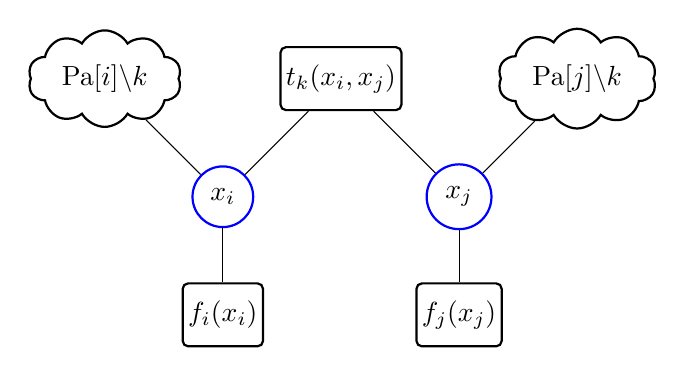
\begin{tikzpicture}
      % \tikzstyle{enode} = [thick, draw=blue, circle, inner sep = 3pt,
      % align=center]
      \tikzstyle{enode} = [thick, draw=blue, circle, inner sep = 4pt,  align=center]
      \tikzstyle{nnode} = [thick, rectangle, rounded corners = 2pt,minimum size = 0.8cm,draw,inner sep = 2pt]

      \tikzstyle{cnode} = [thick, cloud, draw,cloud puffs=10, cloud puff arc=120, aspect=2, inner ysep=4pt]

      \node[cnode] (pajk) at (3, 1.5) {$\text{Pa}[j]\backslash k$};
      \node[cnode] (paik) at (-3, 1.5) {$\text{Pa}[i]\backslash k$};

      \node[nnode] (tk) at (0, 1.5) {$t_k(x_i, x_j)$};
      \node[enode] (xi) at (-1.5 ,0) {$x_i$};
      \node[nnode] (fi) at (-1.5 , -1.5) {$f_i(x_i)$};

      \node[enode] (xj) at (1.5 ,0) {$x_j$};
      \node[nnode] (fj) at (1.5 , -1.5) {$f_j(x_j)$};
      % connections

      \draw[-] (xi) to (fi);
      \draw[-] (xi) to (tk);
      \draw[-] (xi) to (paik);

      \draw[-] (xj) to (fj);
      \draw[-] (xj) to (tk);
      \draw[-] (xj) to (pajk);
    \end{tikzpicture}
    \caption{Factor graph of the linear model.}\label{fig:factor-graph}
    \vspace{0.1cm}
  \end{centering}
\end{figure}


\subsection{Alpha Belief Propagation}
\subsubsection{Fully Factorized Surrogate}
Now we formulated the approximated posterior
\begin{equation}
  q(\bm{x}) \propto \prod_{{i}} \tilde{f}_i(x_i) \prod_{k\in \text{Pa}[i,j]} \tilde{t}_k(x_i, x_j), \bm{x} \in \Aa^N
\end{equation}
to approximate $p(\bm{x}|\bm{y})$. We further assume that $q(\bm{x})$ can be fully factorized, which means that $\tilde{t}_k(x_i, x_j)$ can be factorized as two independent functions of $x_i, x_j$ respectively. We denote this factorization as
\begin{equation}
  \tilde{t}_k(x_i, x_j) = m_{k\rightarrow i}(x_i) m_{k\rightarrow j}(x_j).
\end{equation}
We use the notation $m_{k\rightarrow i}(x_i)$ to denote the factor as a function of $x_i$ due to the intuitive fact that $m_{k\rightarrow i}$ is also the message from the factor $t_k(x_i, x_j)$ to variable node $x_i$. Similarly we have factor $m_{k\rightarrow j}(x_j)$. Then the marginal can be formulated straightforwardly as
\begin{equation}
  q_i(x_i) \propto \tilde{f}_i(x_i) \prod_{k\in \text{Pa}[i]} m_{k\rightarrow i}(x_i),
\end{equation}
where $\text{Pa}[i]$ is the index set of all factors $t_k(x_i, \cdot)$.

\subsubsection{Local $\alpha$-Divergence Minimization}

Now, we are going to use the heuristic scheme to minimize the information loss by using $q(\bm{x})$ to represent $p(\bm{x}|\bm{y})$. The informaiton loss is measured by $\alpha$-divergence $\Dd_{\alpha}(p(\bm{x}|\bm{y}) \| q(\bm{x}))$.

We do factor-wise refinement to update the factors of $q(\bm{x})$ such that $q(\bm{x})$ approaches $p(\bm{x}|\bm{y})$ asymptotically. Without losing generality, we begin to refine factor $\tilde{t}_k(x_i, x_j)$. Define $q^{\backslash t_k}(\bm{x})$ as all other factors except for $\tilde{t}_k(x_i, x_j)$
\begin{align}
  q^{\backslash k}(\bm{x}) &= q(\bm{x})/\tilde{t}_k(x_i, x_j) \nonumber \\
                           &\propto \prod_{{i}} \tilde{f}_i(x_i) \prod_{n\in \text{Pa}[i,j] \backslash k} \tilde{t}_n(x_i, x_j)
\end{align}

Similarly, we have $p^{\backslash k}(\bm{x}|\bm{y})$ as all other factors except for $t_k(x_i, x_j)$. Assume that we already have had $q^{\backslash k}(\bm{x})$ as a good approximation of $p^{\backslash k}(\bm{x}|\bm{y})$, i.e. $q^{\backslash k}(\bm{x}) \simeq p^{\backslash k}(\bm{x}|\bm{y})$, it is $\tilde{t}_k(x_i, x_j)$ remaining to be refined. 
Then it is up to solve
\begin{equation}
  \uargmin{\tilde{t}_k^{\text{new}}(x_i, x_j)} \Dd_{\alpha}\left(  q^{\backslash k}(\bm{x}) t_k(x_i, x_j)\|q^{\backslash k}(\bm{x}) \tilde{t}_k^{\text{new}}(x_i, x_j) \right)
\end{equation}


Using \autoref{eq:fixed-point-iter}, the above problem is equivalent to

\begin{align}\label{eq:update-rule}
  &q^{\backslash t_k}(\bm{x}) \tilde{t}_k^{\text{new}}(x_i, x_j) \nonumber\\
  &\propto \text{proj}\left[ \left(q^{\backslash t_k}(\bm{x}) t_k(x_i, x_j)  \right)^{\alpha} \left(q^{\backslash t_k}(\bm{x}) \tilde{t}_k(x_i, x_j)  \right)^{1-\alpha} \right] \nonumber \\
  & \propto \text{proj}\left[ q^{\backslash t_k}(\bm{x}) t_k(x_i, x_j)^{\alpha} \tilde{t}_k(x_i, x_j)^{1-\alpha} \right]
\end{align}

Let us refine one message per time, i.e.
\begin{equation}
  \tilde{t}_k^{\text{new}}(x_i, x_j) = m_{k\rightarrow i}^{\text{new}}(x_i) m_{k\rightarrow j}(x_j)
\end{equation}

Since the KL-projection to a fully factorized distribution reduces to matching the marginals, the \autoref{eq:update-rule} is reduced to
\begin{equation}\label{eq:message-update}
  \sum_{\bm{x}\backslash x_i} q^{\backslash t_k}(\bm{x}) \tilde{t}_k^{\text{new}}(x_i, x_j) \propto \sum_{\bm{x}\backslash x_i} q^{\backslash t_k}(\bm{x}) \tilde{t}_k(x_i, x_j)
\end{equation}
Reformulating \autoref{eq:message-update} gives the message passing rule as
\begin{align}\label{eq:message-rule}
  {m}^{\text{new}}_{k\rightarrow i}(x_i) \propto & m_{k\rightarrow i}(x_i)^{1-\alpha} \sum_{x_j} \tilde{f}_j(x_j) t_k(x_i, x_j)^{\alpha}\nonumber \\
                                                 &{m}_{k\rightarrow j}(x_j)^{1-\alpha} \prod_{n \in \text{Pa}[j] \backslash k} m_{n \rightarrow j}(x_j).
\end{align}
Similarly, the message from $t_k$ to $x_j$, $m_{k \rightarrow j}(x_j)$, can be updated as $m_{k \rightarrow i}(x_i)$.

Since there is the independent type of factor $\tilde{f}_i(x_i)$ apart from factor $\tilde{t}_k(x_i, x_j)$, similar refinement steps can be carried out as the way we update $\tilde{t}_k$. This gives us the update rule of $\tilde{f}_i(x_i)$ as
\begin{equation}
  \tilde{f}_i^{\text{new}}(x_i) \propto f_i(x_i)^{\alpha} \tilde{f}_i(x_i)^{1-\alpha},
\end{equation}
which is the belief from factor $f_i(x_i)$ to variable $x_i$. Note, if we initialize $\tilde{f}_i(x_i) = f_i(x_i)$, then it reminds the same all the time.

\textcolor{red}{maybe a algorithm box here}
\subsection{Remarks on $\alpha$-BP}\label{subsec:remark}
\begin{figure}[!ht]
  \begin{centering}
    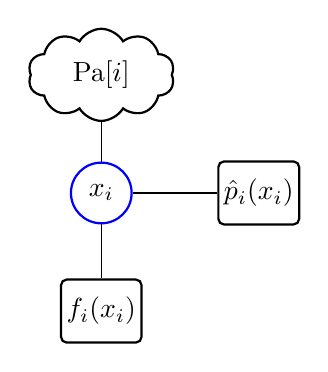
\begin{tikzpicture}
      % \tikzstyle{enode} = [thick, draw=blue, circle, inner sep = 3pt,
      % align=center]
      \tikzstyle{enode} = [thick, draw=blue, circle, inner sep = 4pt,  align=center]
      \tikzstyle{nnode} = [thick, rectangle, rounded corners = 2pt,minimum size = 0.8cm,draw,inner sep = 2pt]

      \tikzstyle{cnode} = [thick, cloud, draw,cloud puffs=10, cloud puff arc=120, aspect=2, inner ysep=4pt]

      \node[cnode] (paik) at (0, 1.5) {$\text{Pa}[i]$};

      \node[enode] (xi) at (0 ,0) {$x_i$};
      \node[nnode] (fi) at (0 , -1.5) {$f_i(x_i)$};
      \node[nnode] (pi) at (2, 0) {$\hat{p}_i(x_i)$};
      % connections
      \draw[-] (xi) to (fi);
      \draw[-] (xi) to (pi);
      \draw[-] (xi) to (paik);
    \end{tikzpicture}
    \caption{Factor graph of the linear model with prior factor.}\label{fig:factor-graph-with-prior}
    \vspace{0.1cm}
  \end{centering}
\end{figure}

As said in \autoref{sec:preliminary}, $KL(p\|q)$ is the special case of $\Dd_{\alpha}(p\|q)$ when $\alpha = 1$. When applying $\alpha=1$ to \autoref{eq:message-rule}, it gives

\begin{equation}\label{eq:message-rule}
  {m}^{\text{new}}_{k\rightarrow i}(x_i) \propto \sum_{x_j} \tilde{f}_j(x_j) t_k(x_i, x_j) \prod_{n \in \text{Pa}[j] \backslash k} m_{n \rightarrow j}(x_j),
\end{equation}
which is exactly the messages in standard belief propagation in Chapter~$8$ of \cite{Bishop:2006:PRM:1162264}. From this point of view, $\alpha$-BP generalizes BP.

Inspired by \cite{pseudo_priorBP2010}, and assembling methods[], we can add an extra independent factor to each $x_i$ as prior information obtained from other (usually weak) estimator. This factor stands for our belief from exterior estimation. Then run our $\alpha$-BP. Denote the prior by $p(x_i)$ for variable node $x_i$, then the factor graph including this prior can be represented in \autoref{fig:factor-graph-with-prior}.

\section{Experimental Results}
In this section, we report numerical results on the $\alpha$-BP. It is well known the performance of BP and its variants deteriorate significantly when loops appear in factor graph. We are curious about if this also affecting $\alpha$-BP. Thus we firstly test the performance of $\alpha$-BP for MAP inference in a binary Markov random field (MRF), where we manipulate how loopy its corresponding factor graph is.

In addition, we apply the $\alpha$-BP to a MIMO detection problem which corresponds to the linear problem in \autoref{eq:linear-model}, to explore its performance in comparison with standard BP and MMSE. At the end, the prior factor trick is used where use the estimation from MMSE to form the prior factor and then run $\alpha$-BP.


\subsection{$\alpha$-BP on MRF}
\begin{figure}[!ht]
  \captionsetup[subfigure]{justification=centering}
  \centering
  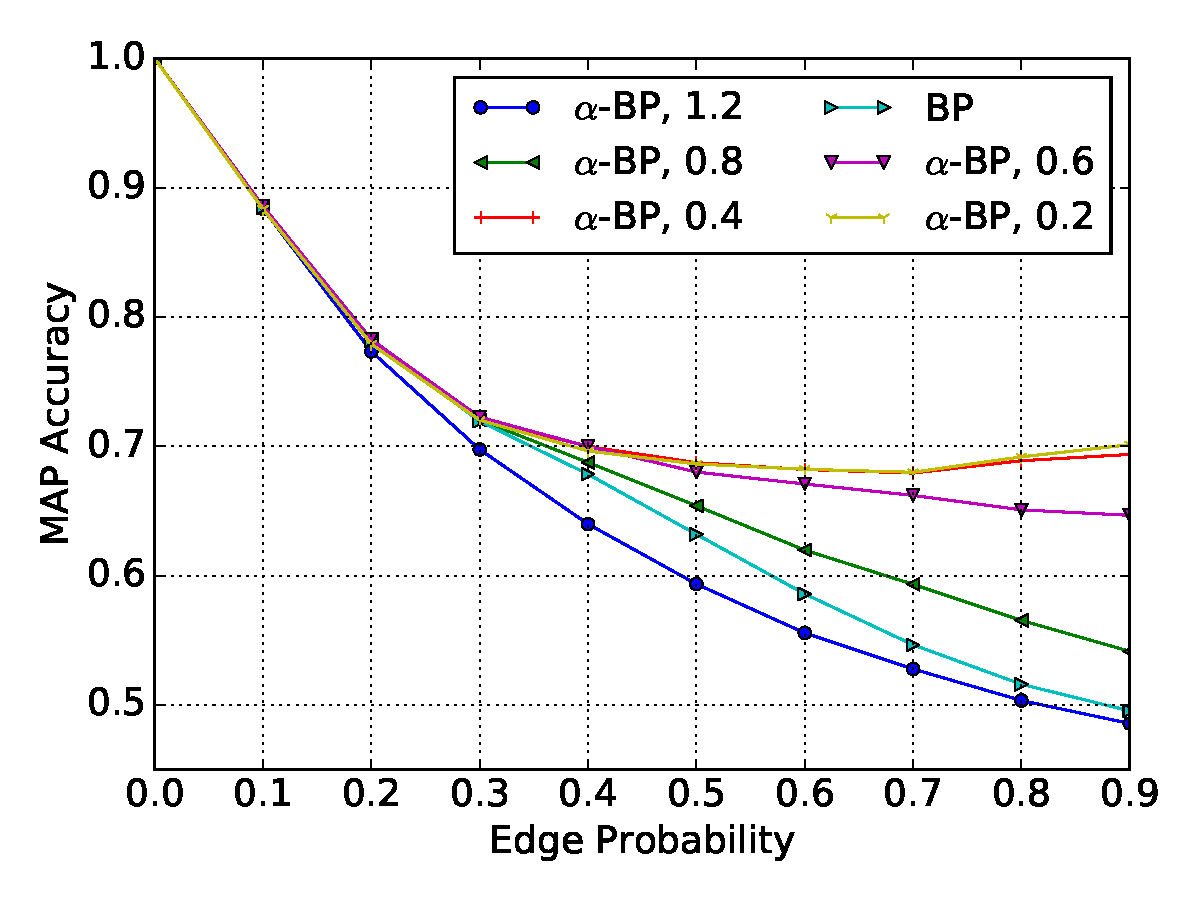
\includegraphics[width=1\linewidth]{figures/MAPacc_edgeP_sum.pdf}
  \caption{Mismatch between MAP and $\alpha$-BP}
  \label{fig:mismatch}
\end{figure}

A MRF has probabilistic distribution $p(\bm{x}) \propto \exp\{-\bm{x}^{T}\bm{J}\bm{x} - \bm{b}^{T}\bm{x}\}$, $\bm{x} \in \Aa^N$. For this experiments, we set $\Aa = \left\{ -1, 1 \right\}$ and $N=9$. Bias $\bm{b}$ is sampled from Gaussian, ${b_i} \sim \Nn(0, (1/4)^2)$. Since $\bm{J}$ decides the loopy level of its corresponding factor graph, we use the Erdos-R�nyi model \cite{erdos1960} to construct its connectivity. Namely, an element of $\bm{J}$ is set as non-zero, $ \bm{J}_{i,j} = \bm{J}_{j,i} \sim \Nn(0,1)$, with a \textit{Edge Probability}. Otherwise, $\bm{J}_{i, j} = \bm{J}_{j,i} = 0$, which means this is no connection between variable node $x_i$ and $x_j$. For each test value of Edge Probability, $5000$ binary MRF models are generated randomly and mismatch between $\argmax_{\bm{x}} p(\bm{x})$ and $\left\{ \bm{x}|\argmax_{x_i}q_i(x_i) \right\}$. The results are shown in \autoref{fig:mismatch}. As the Edge Probability increases, graphs become loopier and $\alpha$-BP (also BP) has more mismatch with MAP inference. In general, $\alpha$-BP with $\alpha > 1$ underperforms BP, and $\alpha$-BP with $\alpha < 1$ outperforms BP. For $\alpha=0.2, 0.4, 0.6$, $\alpha$-BP stops deteriorating for Edge Probability increasing over $0.35$, while BP continues giving even worse approximations.


\subsection{Application to MIMO Detection}
\begin{figure}[!ht]
  \captionsetup[subfigure]{justification=centering}
  \centering
  \begin{subfigure}{.5\textwidth}
    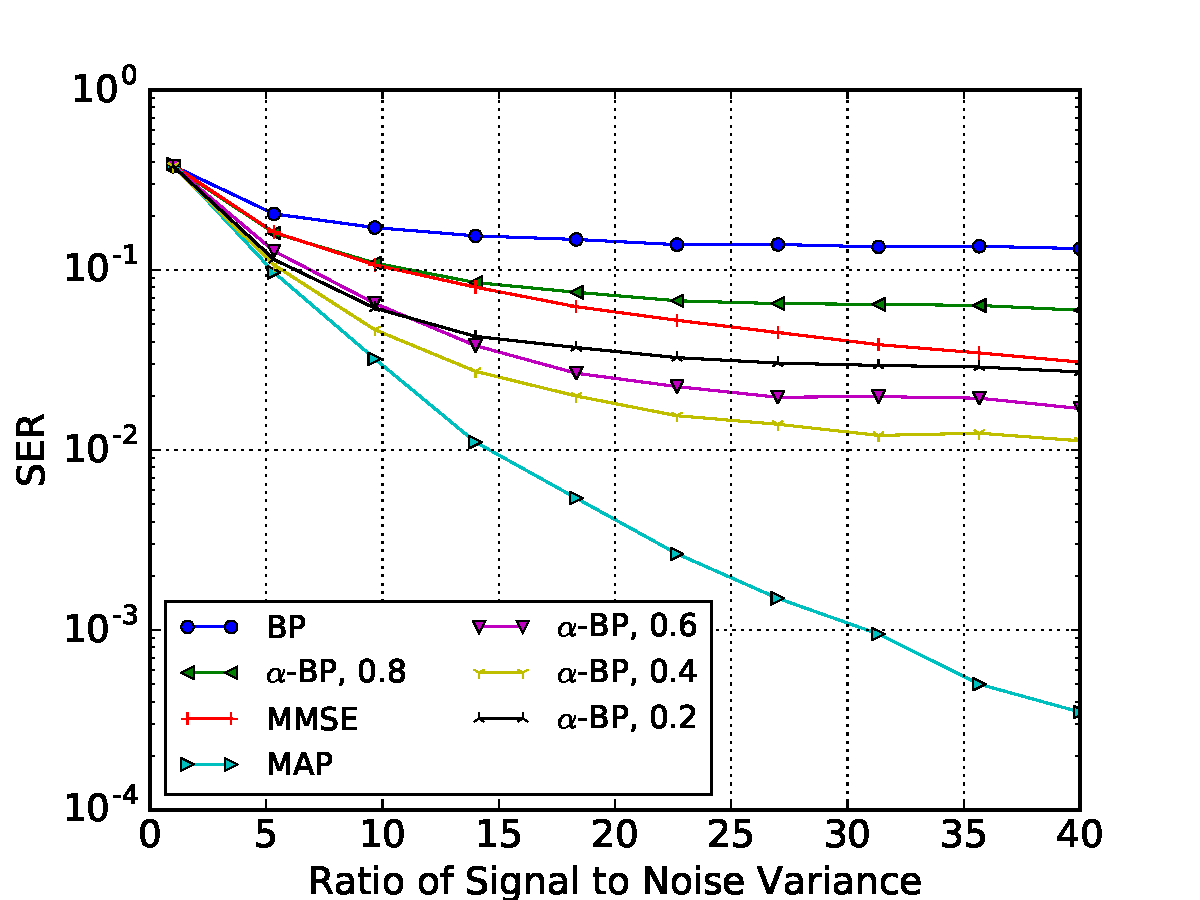
\includegraphics[width=1\linewidth]{figures/alpha_compare.pdf}
    \caption{Without Prior}\label{fig:mimo_a}
  \end{subfigure}
  \centering
  \begin{subfigure}{.5\textwidth}
    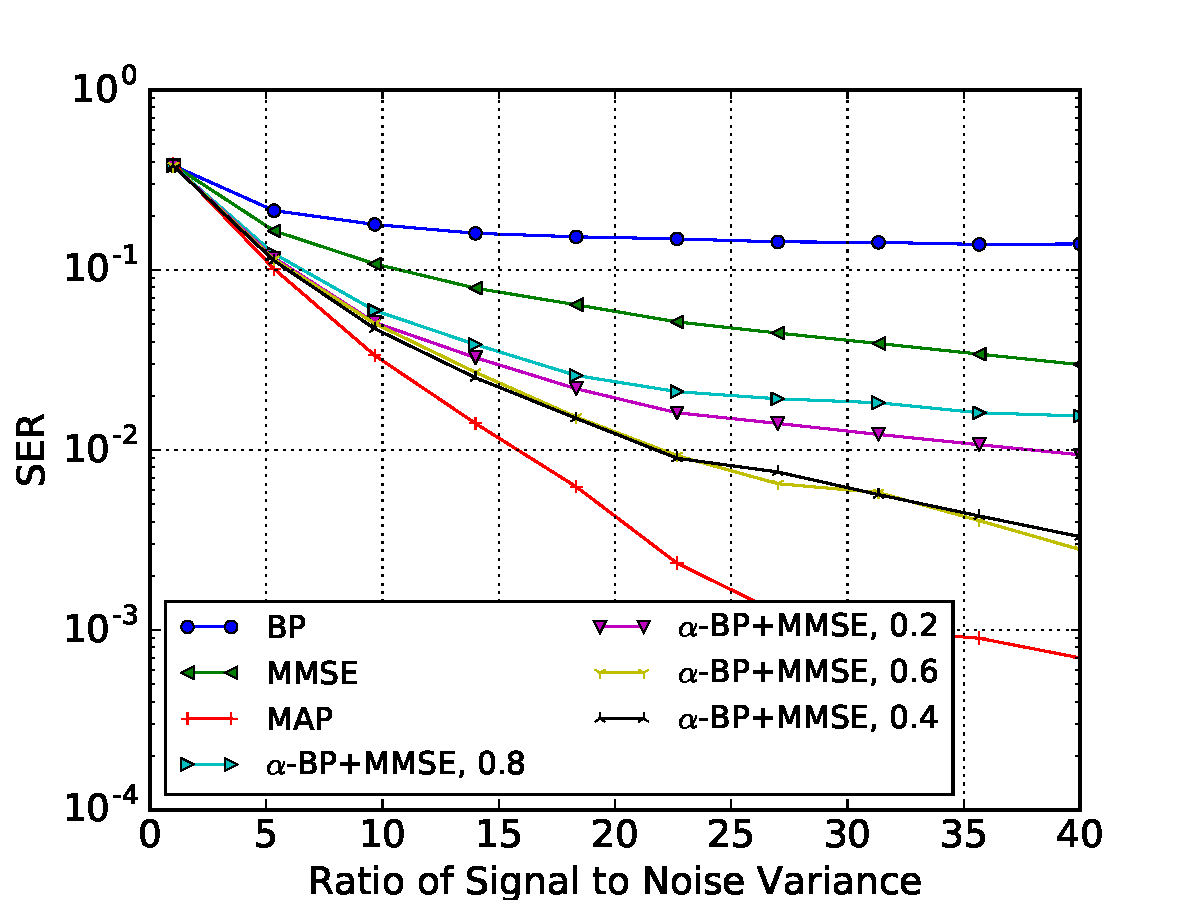
\includegraphics[width=1\linewidth]{figures/prior_mmse_alpha_compare.pdf}
    \caption{With Prior}\label{fig:mimo_b}
  \end{subfigure}
  \caption{MIMO detection in Comparison with MMSE and MAP: (a). $\alpha$-BP without prior; (b). $\alpha$-BP with prior from MMSE.}
  \label{fig:mimo_detection}
\end{figure}

In \autoref{fig:mimo_detection}, we test the application of $\alpha$-BP to MIMO signal detection, which exactly corresponds to the linear model \autoref{eq:linear-model}. In this case, $\bm{y}$ is the received signal, $\bm{H}$ represents the channel gain, and $\bm{e}$ is the white noise. We set $\Aa = \left\{ -1, 1 \right\}$, $N = 8$, and $\bm{H}\in \RR^{8 \times 8}$ sampled from Gaussian.

We run the $\alpha$-BP, with \autoref{fig:mimo_a} and without prior \autoref{fig:mimo_b} (legend ``$\alpha$-BP$+$MMSE'') from MMSE. The reference results of MMSE and MAP inference are also reported under the same conditions. MMSE estimator gives Gaussian posterior $\Nn(\hat{\bm{\mu}}, \hat{\bm{\Sigma}})$ with $\hat{\bm{\mu}} = (\bm{H}^{T}\bm{H} + \sigma_w^2 \bm{I})^{-1}\bm{H}^{T}\bm{y}$ and $\hat{\bm{\Sigma}} = (\bm{H}^{T}\bm{H} + \sigma_w^2 \bm{I})^{-1}\sigma_w$. \autoref{fig:mimo_a} shows that standard BP even underperforms MMSE but $\alpha$-BP can outperform MMSE by assigning smaller value of $\alpha$.

Note that MMSE requires the matrix inverse computation whose complexity increases as $N$ is large. $\alpha$-BP avoid this problem and still can outperform MMSE. But there is still a big gap between $\alpha$-BP (even for $\alpha=0.4$) and MAP. This gap be decreased further by using the prior trick discussed in \autoref{subsec:remark}. \autoref{fig:mimo_b} exemplifies this effects by using prior belief from MMSE, $\hat{p}_i(x_i)\propto \exp\{-(x_i-\mu_i)^2/(2\Sigma_{i,i})\}$. The legend is "$\alpha$-BP$+$MMSE".

\section{Conclusion}
In this work, we obtain the $\alpha$-BP method by doing local $\alpha$-divergence minimization between model distribution $p$ and surrogate distribution $q$. $\alpha$-BP is a practical Bayesian method for message passing. $\alpha$-BP performs well in most probable estimation. With prior trick, $\alpha$-BP performance can be further improved. Future works would be to investigate the parallel message passing of $\alpha$-BP to do difference factor refining currently. It is also interesting to study guideline on choice of $\alpha$.

\bibliographystyle{plain}

% \bibliography{bibliography}
\bibliography{myref}

% \appendix

% \input{section/sec-appendixA}
\end{document}

%%% Local Variables:
%%% mode: latex
%%% TeX-master: t
%%% End:
